% Options for packages loaded elsewhere
\PassOptionsToPackage{unicode}{hyperref}
\PassOptionsToPackage{hyphens}{url}
\PassOptionsToPackage{dvipsnames,svgnames*,x11names*}{xcolor}
%
\documentclass[
  10pt,
  ignorenonframetext,
  aspectratio=43,
]{beamer}
\usepackage{pgfpages}
\setbeamertemplate{caption}[numbered]
\setbeamertemplate{caption label separator}{: }
\setbeamercolor{caption name}{fg=normal text.fg}
\beamertemplatenavigationsymbolsempty

%%
%%% Definition of colors
%%% Source: https://latexcolor.com/
\definecolor{blanchedalmond}{rgb}{1.0, 0.92, 0.8}
\definecolor{blond}{rgb}{0.98, 0.94, 0.75}
%%% End of definition of colors
%%

% Prevent slide breaks in the middle of a paragraph
\widowpenalties 1 10000
\raggedbottom
\usepackage{lmodern}
\usepackage{amssymb,amsmath}
\usepackage{ifxetex,ifluatex}
\ifnum 0\ifxetex 1\fi\ifluatex 1\fi=0 % if pdftex
  \usepackage[T1]{fontenc}
  \usepackage[utf8]{inputenc}
  \usepackage{textcomp} % provide euro and other symbols
\else % if luatex or xetex
  \usepackage{unicode-math}
  \defaultfontfeatures{Scale=MatchLowercase}
  \defaultfontfeatures[\rmfamily]{Ligatures=TeX,Scale=1}
  \setmainfont[]{Myriad Pro}
  \ifxetex
    \usepackage{xeCJK}
    \setCJKmainfont[ItalicFont=AR PL UKai TW]{AR UDJingXiHeiPU30}
  \fi
  \ifluatex
    \usepackage[]{luatexja-fontspec}
    \setmainjfont[ItalicFont=AR PL UKai TW]{AR UDJingXiHeiPU30}
  \fi
\fi
\usetheme[]{metropolis}
\usecolortheme{default}
\usefonttheme{serif} % use mainfont rather than sansfont for slide text
% Use upquote if available, for straight quotes in verbatim environments
\IfFileExists{upquote.sty}{\usepackage{upquote}}{}
\IfFileExists{microtype.sty}{% use microtype if available
  \usepackage[]{microtype}
  \UseMicrotypeSet[protrusion]{basicmath} % disable protrusion for tt fonts
}{}
\makeatletter
\@ifundefined{KOMAClassName}{% if non-KOMA class
  \IfFileExists{parskip.sty}{%
    \usepackage{parskip}
  }{% else
    \setlength{\parindent}{0pt}
    \setlength{\parskip}{6pt plus 2pt minus 1pt}}
}{% if KOMA class
  \KOMAoptions{parskip=half}}
\makeatother
\usepackage{xcolor}
\IfFileExists{xurl.sty}{\usepackage{xurl}}{} % add URL line breaks if available
\IfFileExists{bookmark.sty}{\usepackage{bookmark}}{\usepackage{hyperref}}
\hypersetup{
  pdftitle={Reserving Female Status --- Women Reserved Seats and Gender Empowerment in Taiwan},
  pdfauthor={Yu-Hsin Ho},
  colorlinks=true,
  linkcolor=Maroon,
  filecolor=Maroon,
  citecolor=Blue,
  urlcolor=red,
  pdfcreator={LaTeX via pandoc}}
\urlstyle{same} % disable monospaced font for URLs
\newif\ifbibliography
\usepackage{listings}
\newcommand{\passthrough}[1]{#1}
\lstset{defaultdialect=sh}
\lstset{framexleftmargin=0mm, frame=trBL,backgroundcolor=\color{blanchedalmond!5},numbers=left,numberstyle=\scriptsize,basicstyle=\small}
\lstset{aboveskip=5mm,belowskip=5mm,xleftmargin=20pt,xrightmargin=5pt}
% \lstset{prebreak={\raisebox{0ex}[0ex][0ex]}}
% \lstset{postbreak={\raisebox{0ex}[0ex][0ex]\space}}
\lstset{breaklines=true,breakatwhitespace=true}
\usepackage{longtable,booktabs}
\setlength{\emergencystretch}{3em} % prevent overfull lines
\providecommand{\tightlist}{%
  \setlength{\itemsep}{0pt}\setlength{\parskip}{0pt}}
\setcounter{secnumdepth}{-\maxdimen} % remove section numbering

%
% When using babel or polyglossia with biblatex, loading csquotes is recommended 
% to ensure that quoted texts are typeset according to the rules of your main language.
%
\usepackage{csquotes}

%
% blockquote
%
\definecolor{blockquote-border}{RGB}{221,221,221}
\definecolor{blockquote-text}{RGB}{89,89,89}
\usepackage{mdframed}
\newmdenv[rightline=false,bottomline=false,topline=false,linewidth=3pt,linecolor=blockquote-border,skipabove=\parskip]{customblockquote}
\renewenvironment{quote}{\begin{customblockquote}\list{}{\rightmargin=0em\leftmargin=0em}%
\item\relax\color{blockquote-text}\ignorespaces}{\unskip\unskip\endlist\end{customblockquote}}

%
% Source Sans Pro as the de­fault font fam­ily
% Source Code Pro for monospace text
%
% 'default' option sets the default 
% font family to Source Sans Pro, not \sfdefault.
%

\usepackage{tikz}
\usepackage{pgfplots}
\usepackage{adjustbox}
\usepackage{booktabs}
\linespread{1.3}

\title{Reserving Female Status --- Women Reserved Seats and Gender
Empowerment in Taiwan}
\author{Yu-Hsin Ho}
\date{March 18, 2022}
\institute{Department of Economics, National Taiwan University}

\begin{document}
\frame{\titlepage}

\begin{frame}
  \tableofcontents[hideallsubsections]
\end{frame}
\hypertarget{background}{%
\section{Background}\label{background}}

\begin{frame}{A Progressive Gender Perspective of \emph{ROC
Consitution}}
\protect\hypertarget{a-progressive-gender-perspective-of-roc-consitution}{}
\begin{quote}
\emph{中華民國憲法第 134 條}

各種選舉,應規定婦女當選名額,其辦法以法律定之。
\end{quote}

\begin{itemize}
\tightlist
\item
  Mandatory women reserved seats in \emph{any} election codified in
  \emph{ROC Constitution} since 1946

  \begin{itemize}
  \tightlist
  \item
    Established long before new left feminism movement in 1960s Western
    world
  \item
    Mainly Influenced by May Fourth Movement(新文化運動)and KMT-CCP
    Alliance(聯俄容共)(黃長玲,2012)
  \end{itemize}
\end{itemize}
\end{frame}

\begin{frame}
Past researches on effects of women political representation utilized a
natural experiment in India

\begin{block}{1993 Constitution Amendment in India}
\protect\hypertarget{constitution-amendment-in-india}{}
\begin{itemize}
\tightlist
\item
  1/3 seats reserved for women in local council elections
\item
  Higher female political representation due to this policy
\item
  \textbf{Identification}: States adopting this policy was designated
  randomly, causing random treatment and time variation
\end{itemize}

Outcomes: son preference, crime against women, educational
attainment/investment, gender attitudes, etc.
\end{block}
\end{frame}

\begin{frame}
\begin{itemize}
\tightlist
\item
  Local council elections in Taiwan reserved 1 woman seat per 4 elected
  member

  \begin{itemize}
  \tightlist
  \item
    Guaranteeing 14\% \textasciitilde{} 25\% female representatives for
    electoral districts having \(\geq\) 4 members
  \end{itemize}
\item
  If the number of female elected doesn't meet the requirement, then the
  lowest voted male winner will be replaced by highest voted female
  candidate.
\item
  This provides neater identification of policy effect than India
\end{itemize}
\end{frame}

\begin{frame}{Main Question}
\protect\hypertarget{main-question}{}
\begin{itemize}
\tightlist
\item
  Effects of women reserved seats on \textbf{female political
  representation}
\item
  And its corresponding effects on \textbf{female social status}
\end{itemize}
\end{frame}

\hypertarget{data-and-identification-strategy}{%
\section{Data and Identification
Strategy}\label{data-and-identification-strategy}}

\begin{frame}{Treatment}
\protect\hypertarget{treatment}{}
\(\text{Elected Female \% } E_{tde} = \frac{\text{Female Member Size 女性當選人數}}{\text{Member Size 應選人數}}\)
in year \(t\), period \(e\), and electoral district \(d\).

Data gathered from the City Council Elections:

\begin{itemize}
\tightlist
\item
  from 1998 to 2018 (6 periods in total)
\item
  electoral district level
\end{itemize}

We use IV to deal with endogeneity of \(E_{tde}\), instrumented by the
\% of reserved seats for women \(R_{tde}\).
\end{frame}

\begin{frame}{Instrumenting \(E_{tde}\) by Reserved Seats Proportion
\(R_{tde}\)}
\protect\hypertarget{instrumenting-e_tde-by-reserved-seats-proportion-r_tde}{}
\(\text{Reserved Seats \% } R_{tde} = \frac{\text{Reserved Seats 保留名額數}}{\text{Member Size 應選人數}}\)
in year \(t\), period \(e\), and electoral district \(d\).

\begin{figure}[htb]
\centering
\scalebox{0.7}{
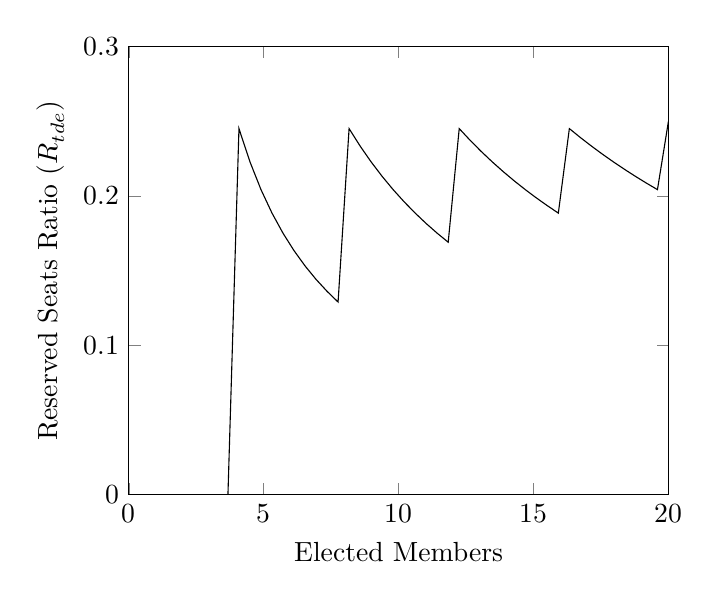
\begin{tikzpicture}
\begin{axis}
[
    xlabel={Elected Members}, 
    ylabel={Reserved Seats Ratio ($R_{tde}$)}, 
    xmin=0, 
    xmax=20, 
    ymin=0, 
    ymax=0.3
]
\addplot[no marks, domain=0:20, samples=50] {floor(x/4)/x};
\end{axis}
\end{tikzpicture}
}
\end{figure}

We capture this discontinuous ``ticks'' as instrument of treatment.
\end{frame}

\begin{frame}{Outcomes}
\protect\hypertarget{outcomes}{}
\begin{block}{1st Stage}
\protect\hypertarget{st-stage}{}
Effects of women reserved seats on \textbf{female political
representativeness}
\end{block}

\begin{block}{2nd Stage}
\protect\hypertarget{nd-stage}{}
Treatment effects on couple's \textbf{son preference}

\begin{itemize}
\tightlist
\item
  Variables:

  \begin{enumerate}
  \tightlist
  \item
    \textbf{Third Child}: Dummy of having 3rd child or not
  \item
    \textbf{Third Child is Son}: Dummy of 3rd child being male
  \end{enumerate}
\item
  Data: Newborns Birth Data 出生人口檔 between 1998 to 2006
\item
  Observation: couple level
\end{itemize}
\end{block}
\end{frame}

\begin{frame}{2SLS Specification}
\protect\hypertarget{sls-specification}{}
2nd Stage: \[
Y_{itde} = \alpha + \beta_1 \hat{E_{tde}} + \gamma_1 \ln \operatorname{population}_{\text{county}} + \delta_t + \delta_{d} + \epsilon_i
\]

1st Stage: \[
\hat{E_{itde}} = \alpha + \beta_1 R_{tde}  + \gamma_1 \ln \operatorname{population}_{\text{county}} + \delta_t + \delta_{d}
\]

Controlling \(\ln \operatorname{population}\) to resolve omitted
variable bias.
\end{frame}

\hypertarget{estimations}{%
\section{Estimations}\label{estimations}}

\begin{frame}{First Stage}
\protect\hypertarget{first-stage}{}
Elasticity of reserved seats on female elected and female candidates are
high.

\begin{table}
    \caption{1st Stage}
    {
        \def\sym#1{\ifmmode^{#1}\else\(^{#1}\)\fi}
        \begin{tabular}{l*{2}{c}}
            \toprule
                               & \multicolumn{1}{c}{(1)}               & \multicolumn{1}{c}{(2)}                  \\
                               & \multicolumn{1}{c}{\% Elected Female} & \multicolumn{1}{c}{\% Female Candidates} \\
            \midrule
            \% Reserved Seats  & 1.029\sym{***}                        & 0.758\sym{***}                           \\
                               & (0.0620)                              & (0.0578)                                 \\
            Population Control & Yes                                   & Yes                                      \\
            Election Year FE   & Yes                                   & Yes                                      \\
            County FE          & Yes                                   & Yes                                      \\
            \midrule
            Observations       & 2210                                  & 2210                                     \\
            \bottomrule
            \multicolumn{3}{l}{\footnotesize Standard errors in parentheses}                                      \\
            \multicolumn{3}{l}{\footnotesize \sym{*} \(p<0.05\), \sym{**} \(p<0.01\), \sym{***} \(p<0.001\)}      \\
        \end{tabular}
    }
\end{table}
\end{frame}

\begin{frame}{Summary of Newborn Data}
\protect\hypertarget{summary-of-newborn-data}{}
\begin{table}[htbp]\centering
    \def\sym#1{\ifmmode^{#1}\else\(^{#1}\)\fi}
    \caption{Summary Statistics of Samples}
    \adjustbox{width=0.7\textwidth}{
        \begin{tabular}{l*{1}{ccccc}}
            \toprule
                        & count  & mean     & sd       & min  & max     \\
            \midrule
            year        & 302972 & 2000.762 & 2.015725 & 1998 & 2006    \\
            byear\_n1   & 302972 & 2000.762 & 2.015725 & 1998 & 2006    \\
            byear\_n2   & 302972 & 2002.895 & 2.112062 & 1998 & 2006    \\
            byear\_n3   & 26532  & 2003.661 & 1.824804 & 1998 & 2006    \\
            sex1        & 302972 & .4973529 & .4999938 & 0    & 1       \\
            sex2        & 302972 & .5256327 & .4993434 & 0    & 1       \\
            sex3        & 26532  & .5505427 & .4974482 & 0    & 1       \\
            thirdChild  & 302972 & .0875724 & .2826726 & 0    & 1       \\
            bachelor\_f & 302972 & .1854264 & .3886437 & 0    & 1       \\
            bachelor\_m & 302972 & .1484197 & .3555161 & 0    & 1       \\
            age\_f      & 302972 & 29.77056 & 4.543678 & 14   & 76      \\
            age\_m      & 302972 & 26.90372 & 4.307737 & 13   & 55      \\
            population  & 302972 & 1577592  & 1034718  & 6560 & 3767095 \\
            \midrule
            \(N\)       & 302972 &          &          &      &         \\
            \bottomrule
        \end{tabular}
    }
\end{table}

\end{frame}

\begin{frame}{Outcome: Son Preference}
\protect\hypertarget{outcome-son-preference}{}
\begin{table}[htbp]\centering
    \def\sym#1{\ifmmode^{#1}\else\(^{#1}\)\fi}
    \caption{2SLS Birth Outcomes of City Council Elections}
    \adjustbox{max width=0.9\textwidth}{
        \begin{tabular}{l*{4}{c}}
            \toprule
                                    & \multicolumn{1}{c}{(1)}              & \multicolumn{1}{c}{(2)}              & \multicolumn{1}{c}{(3)}              & \multicolumn{1}{c}{(4)}              \\
                                    & \multicolumn{1}{c}{Having 3rd Child} & \multicolumn{1}{c}{Having 3rd Child} & \multicolumn{1}{c}{3rd Child is Son} & \multicolumn{1}{c}{3rd Child is Son} \\
            \midrule
            \% Elected Female       & -0.277\sym{***}                      & -0.0460\sym{***}                     & 0.00108                              & 0.0866                               \\
                                    & (0.0237)                             & (0.0122)                             & (0.0576)                             & (0.0594)                             \\
            1 sex                   & -0.0275\sym{***}                     & -0.0273\sym{***}                     & -0.0632\sym{***}                     & -0.0627\sym{***}                     \\
                                    & (0.00111)                            & (0.00110)                            & (0.00595)                            & (0.00594)                            \\
            2 sex                   & -0.0309\sym{***}                     & -0.0309\sym{***}                     & -0.0147\sym{*}                       & -0.0147\sym{*}                       \\
                                    & (0.00117)                            & (0.00115)                            & (0.00622)                            & (0.00623)                            \\
            Parent Age, Edu Control & Yes                                  & Yes                                  & Yes                                  & Yes                                  \\
            Log-Population Control  & Yes                                  & Yes                                  & Yes                                  & Yes                                  \\
            Year FE                 & No                                   & Yes                                  & No                                   & Yes                                  \\
            County FE               & No                                   & Yes                                  & No                                   & Yes                                  \\
            \midrule
            Mean                    & 0.0876                               & 0.0876                               & 0.551                                & 0.551                                \\
            Observations            & 302972                               & 302972                               & 26532                                & 26532                                \\
            Adj. R-square           & 0.00377                              & 0.0305                               & 0.00427                              & 0.00422                              \\
            \bottomrule
            \multicolumn{5}{l}{\footnotesize Standard errors in parentheses}                                                                                                                    \\
            \multicolumn{5}{l}{\footnotesize \sym{*} \(p<0.05\), \sym{**} \(p<0.01\), \sym{***} \(p<0.001\)}                                                                                    \\
        \end{tabular}

    }
\end{table}
\end{frame}

\begin{frame}{Outcome: Subgroup Son Preference}
\protect\hypertarget{outcome-subgroup-son-preference}{}
\begin{table}[htbp]\centering
    \def\sym#1{\ifmmode^{#1}\else\(^{#1}\)\fi}
    \caption{2SLS Subgroup Birth Outcomes of City Council Elections}
    \adjustbox{max width=0.9\textwidth}{
        \begin{tabular}{l*{4}{c}}
            \toprule
                                                           & \multicolumn{1}{c}{(1)}        & \multicolumn{1}{c}{(2)}        & \multicolumn{1}{c}{(3)}               & \multicolumn{1}{c}{(4)}               \\
                                                           & \multicolumn{1}{c}{thirdChild} & \multicolumn{1}{c}{thirdChild} & \multicolumn{1}{c}{third\_child\_son} & \multicolumn{1}{c}{third\_child\_son} \\
            \midrule
            elected\_female\_ratio                         & -0.0697\sym{***}               & 0.0102\sym{**}                 & 0.0587                                & 0.132                                 \\
                                                           & (0.00483)                      & (0.00356)                      & (0.0729)                              & (0.0763)                              \\
            both\_daughter $\times$ elected\_female\_ratio & -0.369\sym{***}                & -0.383\sym{***}                & -0.0477                               & -0.0514                               \\
                                                           & (0.0367)                       & (0.0359)                       & (0.120)                               & (0.120)                               \\
            both\_daughter                                 & 0.182\sym{***}                 & 0.182\sym{***}                 & 0.101\sym{***}                        & 0.102\sym{***}                        \\
                                                           & (0.00804)                      & (0.00798)                      & (0.0245)                              & (0.0245)                              \\
            Population Control                             & Yes                            & Yes                            & Yes                                   & Yes                                   \\
            Year FE                                        & No                             & Yes                            & No                                    & Yes                                   \\
            County FE                                      & No                             & Yes                            & No                                    & Yes                                   \\
            \midrule
            Mean                                           & 0.0176                         & 0.0176                         & 0.554                                 & 0.554                                 \\
            Observations                                   & 1261020                        & 1261020                        & 22229                                 & 22229                                 \\
            Adj. R-square                                  & 0.0253                         & 0.0373                         & 0.00775                               & 0.00813                               \\
            \bottomrule
            \multicolumn{5}{l}{\footnotesize Standard errors in parentheses}                                                                                                                                 \\
            \multicolumn{5}{l}{\footnotesize \sym{*} \(p<0.05\), \sym{**} \(p<0.01\), \sym{***} \(p<0.001\)}                                                                                                 \\
        \end{tabular}
    }
\end{table}

\end{frame}

\begin{frame}{Discussion}
\protect\hypertarget{discussion}{}
\begin{block}{Outcome: 3rd Child}
\protect\hypertarget{outcome-3rd-child}{}
\begin{enumerate}
\tightlist
\item
  Increase Female \textbf{Bargaining Power}

  \begin{itemize}
  \tightlist
  \item
    Only couples with extreme sex composition consider to have 3rd child
  \item
    Decreased willingness to pay additional son/daughter
  \item
    No effects on college graduates (high bargaining power already)
  \end{itemize}
\item
  Weaken \textbf{Son Preference}

  \begin{itemize}
  \tightlist
  \item
    Larger effect on couples without son
  \end{itemize}
\end{enumerate}
\end{block}

\begin{block}{Outcome: Sex ratio of 3rd parity}
\protect\hypertarget{outcome-sex-ratio-of-3rd-parity}{}
\begin{itemize}
\tightlist
\item
  Indicating behaviors of those who had conservative gender attitudes

  \begin{itemize}
  \tightlist
  \item
    Higher willingness to pay for a son
  \end{itemize}
\item
  Sex selection existed, and higher female representation didn't abolish
  it.
\end{itemize}
\end{block}
\end{frame}

\hypertarget{potential-issues}{%
\section{Potential Issues}\label{potential-issues}}

\begin{frame}{Potential Issues}
\begin{block}{Outcomes on Gender Attitudes}
\protect\hypertarget{outcomes-on-gender-attitudes}{}
\begin{itemize}
\tightlist
\item
  Taiwan Social Change Survey
\end{itemize}
\end{block}

\begin{block}{Other Influencing Channels}
\protect\hypertarget{other-influencing-channels}{}
\begin{itemize}
\tightlist
\item
  Elected or Candidacy?
\end{itemize}
\end{block}

\begin{block}{Mechanisms}
\protect\hypertarget{mechanisms}{}
\begin{itemize}
\tightlist
\item
  Role-model effect
\item
  Policy effect

  \begin{itemize}
  \tightlist
  \item
    Labor market outcomes
  \item
    Pro-female policies
  \end{itemize}
\end{itemize}
\end{block}
\end{frame}

\end{document}
